% !TeX root = ../../Skript.tex
\cohead{\Large\textbf{Gegenseitige Lage von Geraden}}
\fakesubsection{Gegenseitige Lage von Geraden}

\begin{minipage}{\textwidth}
	\centering{\Large\textcolor{loes}{Parallele Geraden}}
	\adjustbox{valign=t, padding=0ex 0ex 2ex 0ex}{\begin{minipage}{0.5\linewidth-2ex}\centering
		\centering{\iftoggle{ausfuellen}{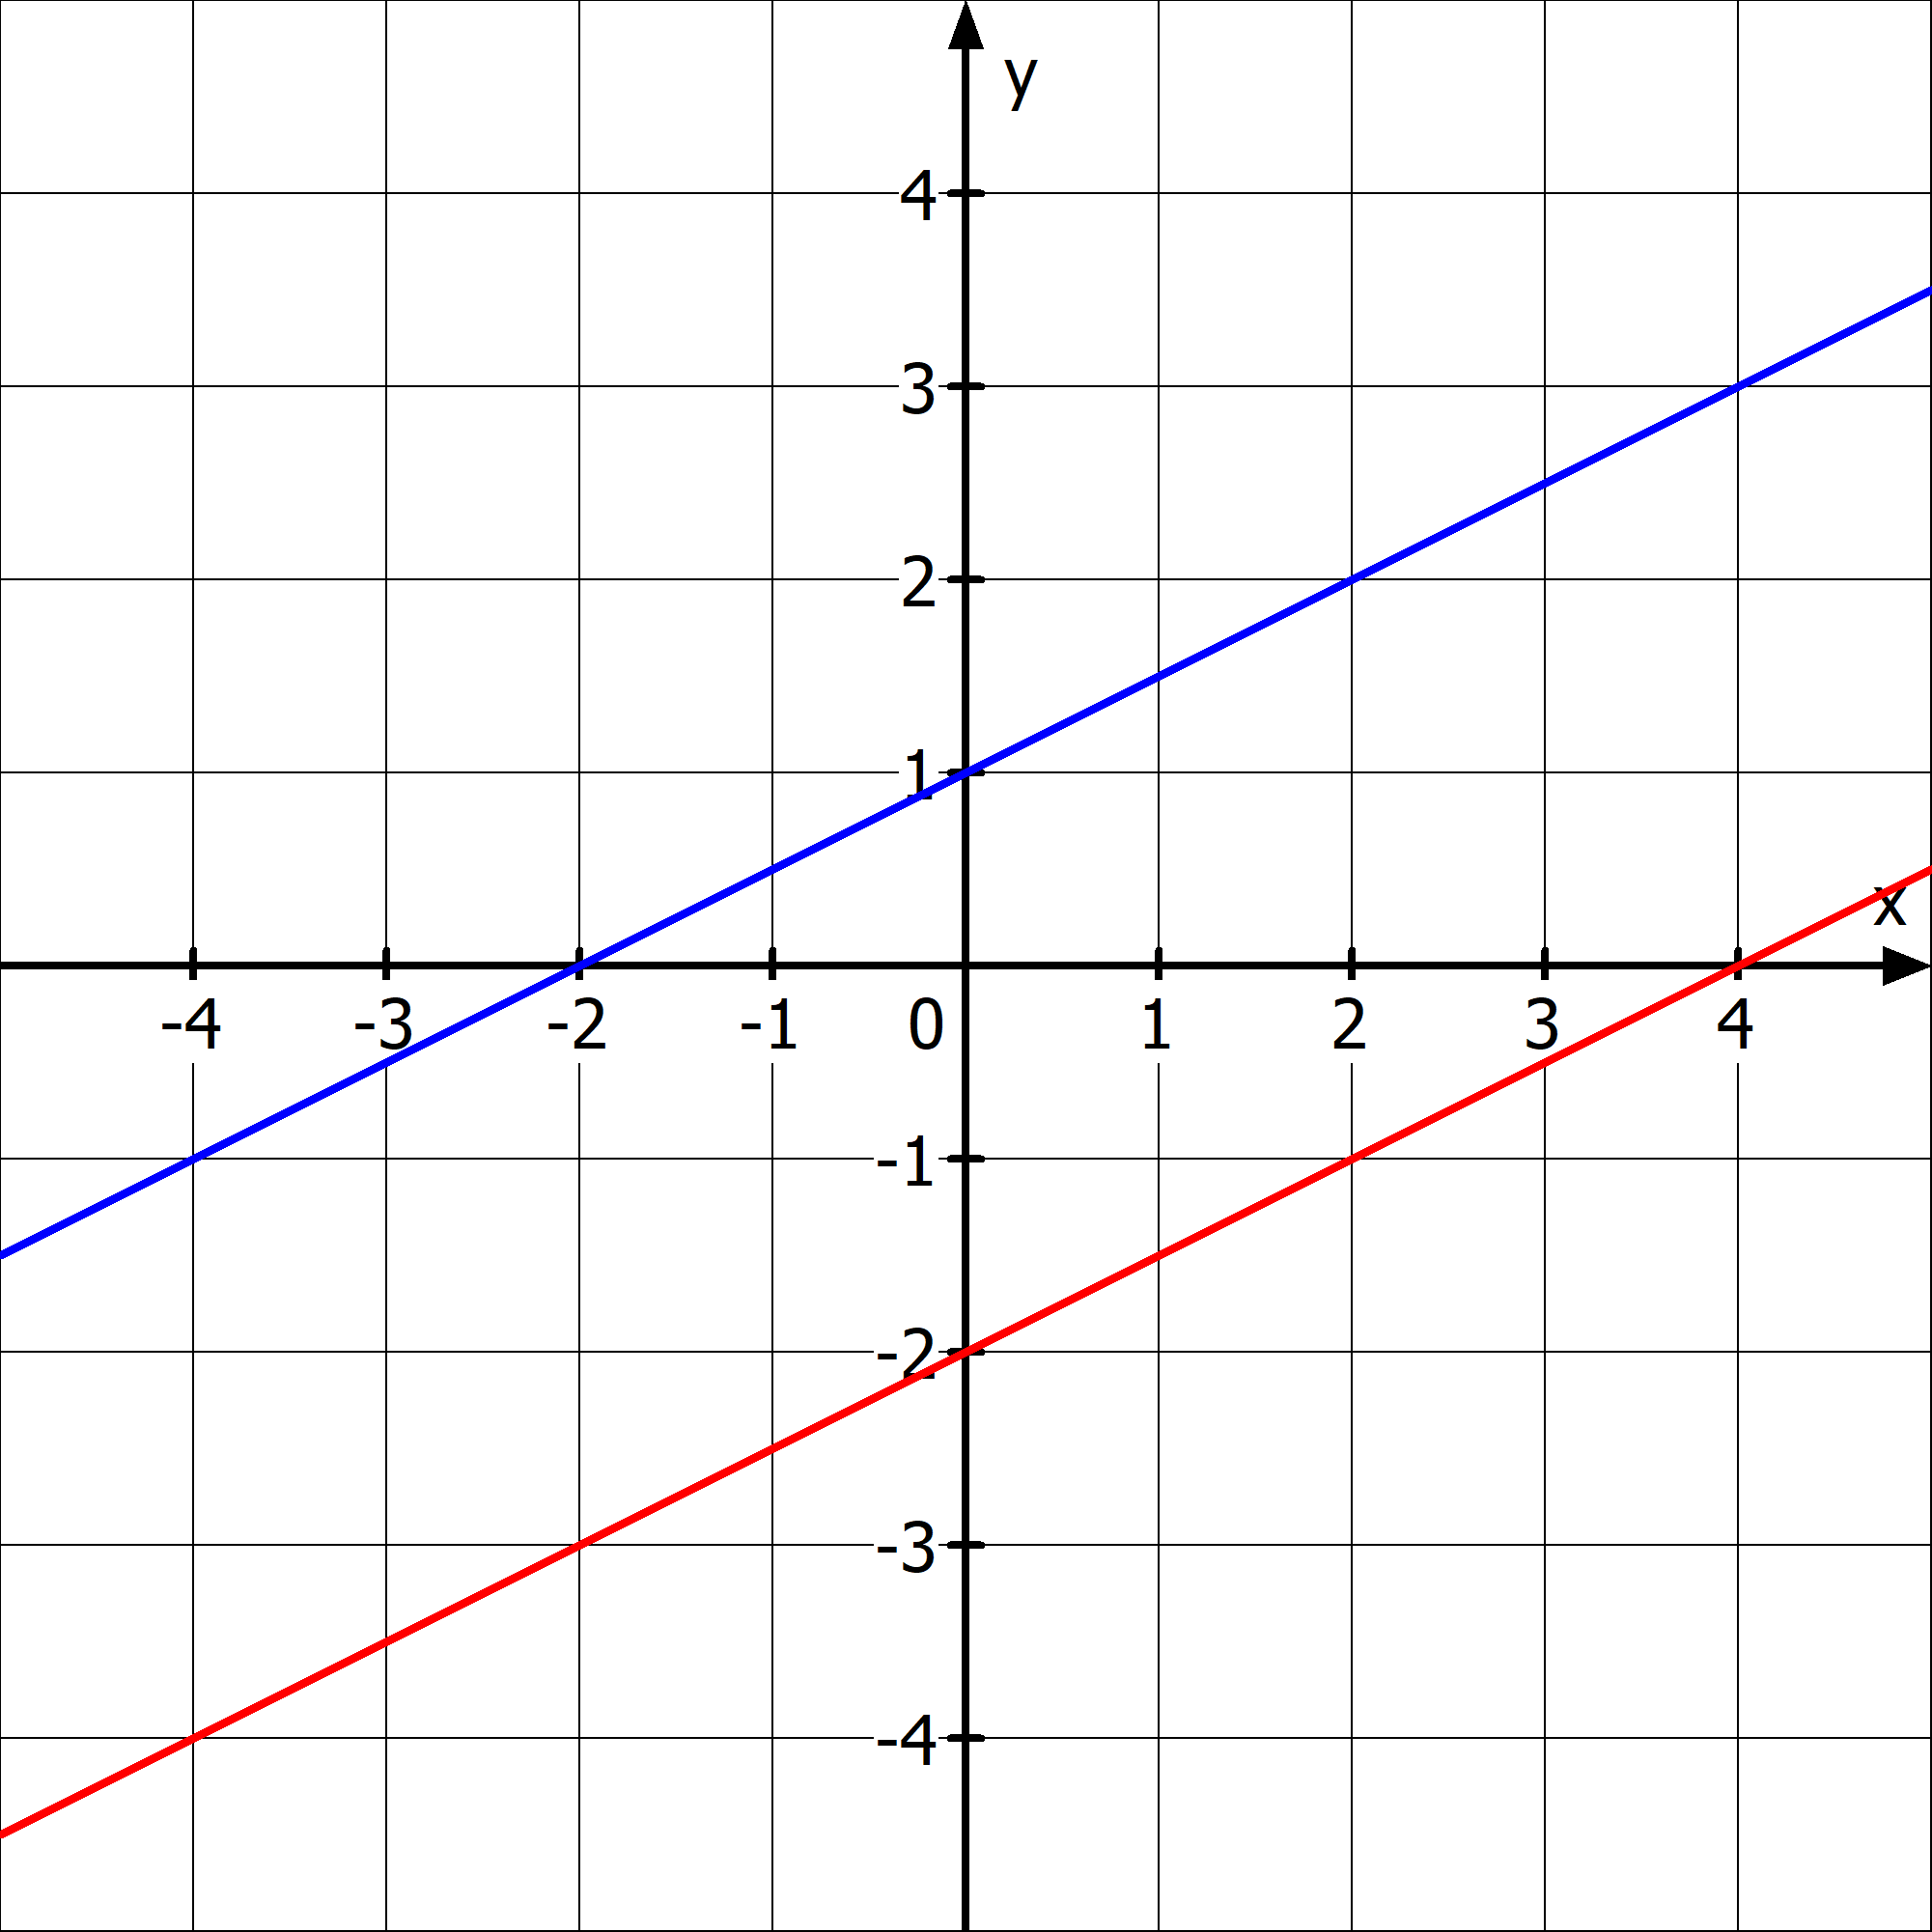
\includegraphics[width=\linewidth]{\linFkt/pics/lage1.png}}{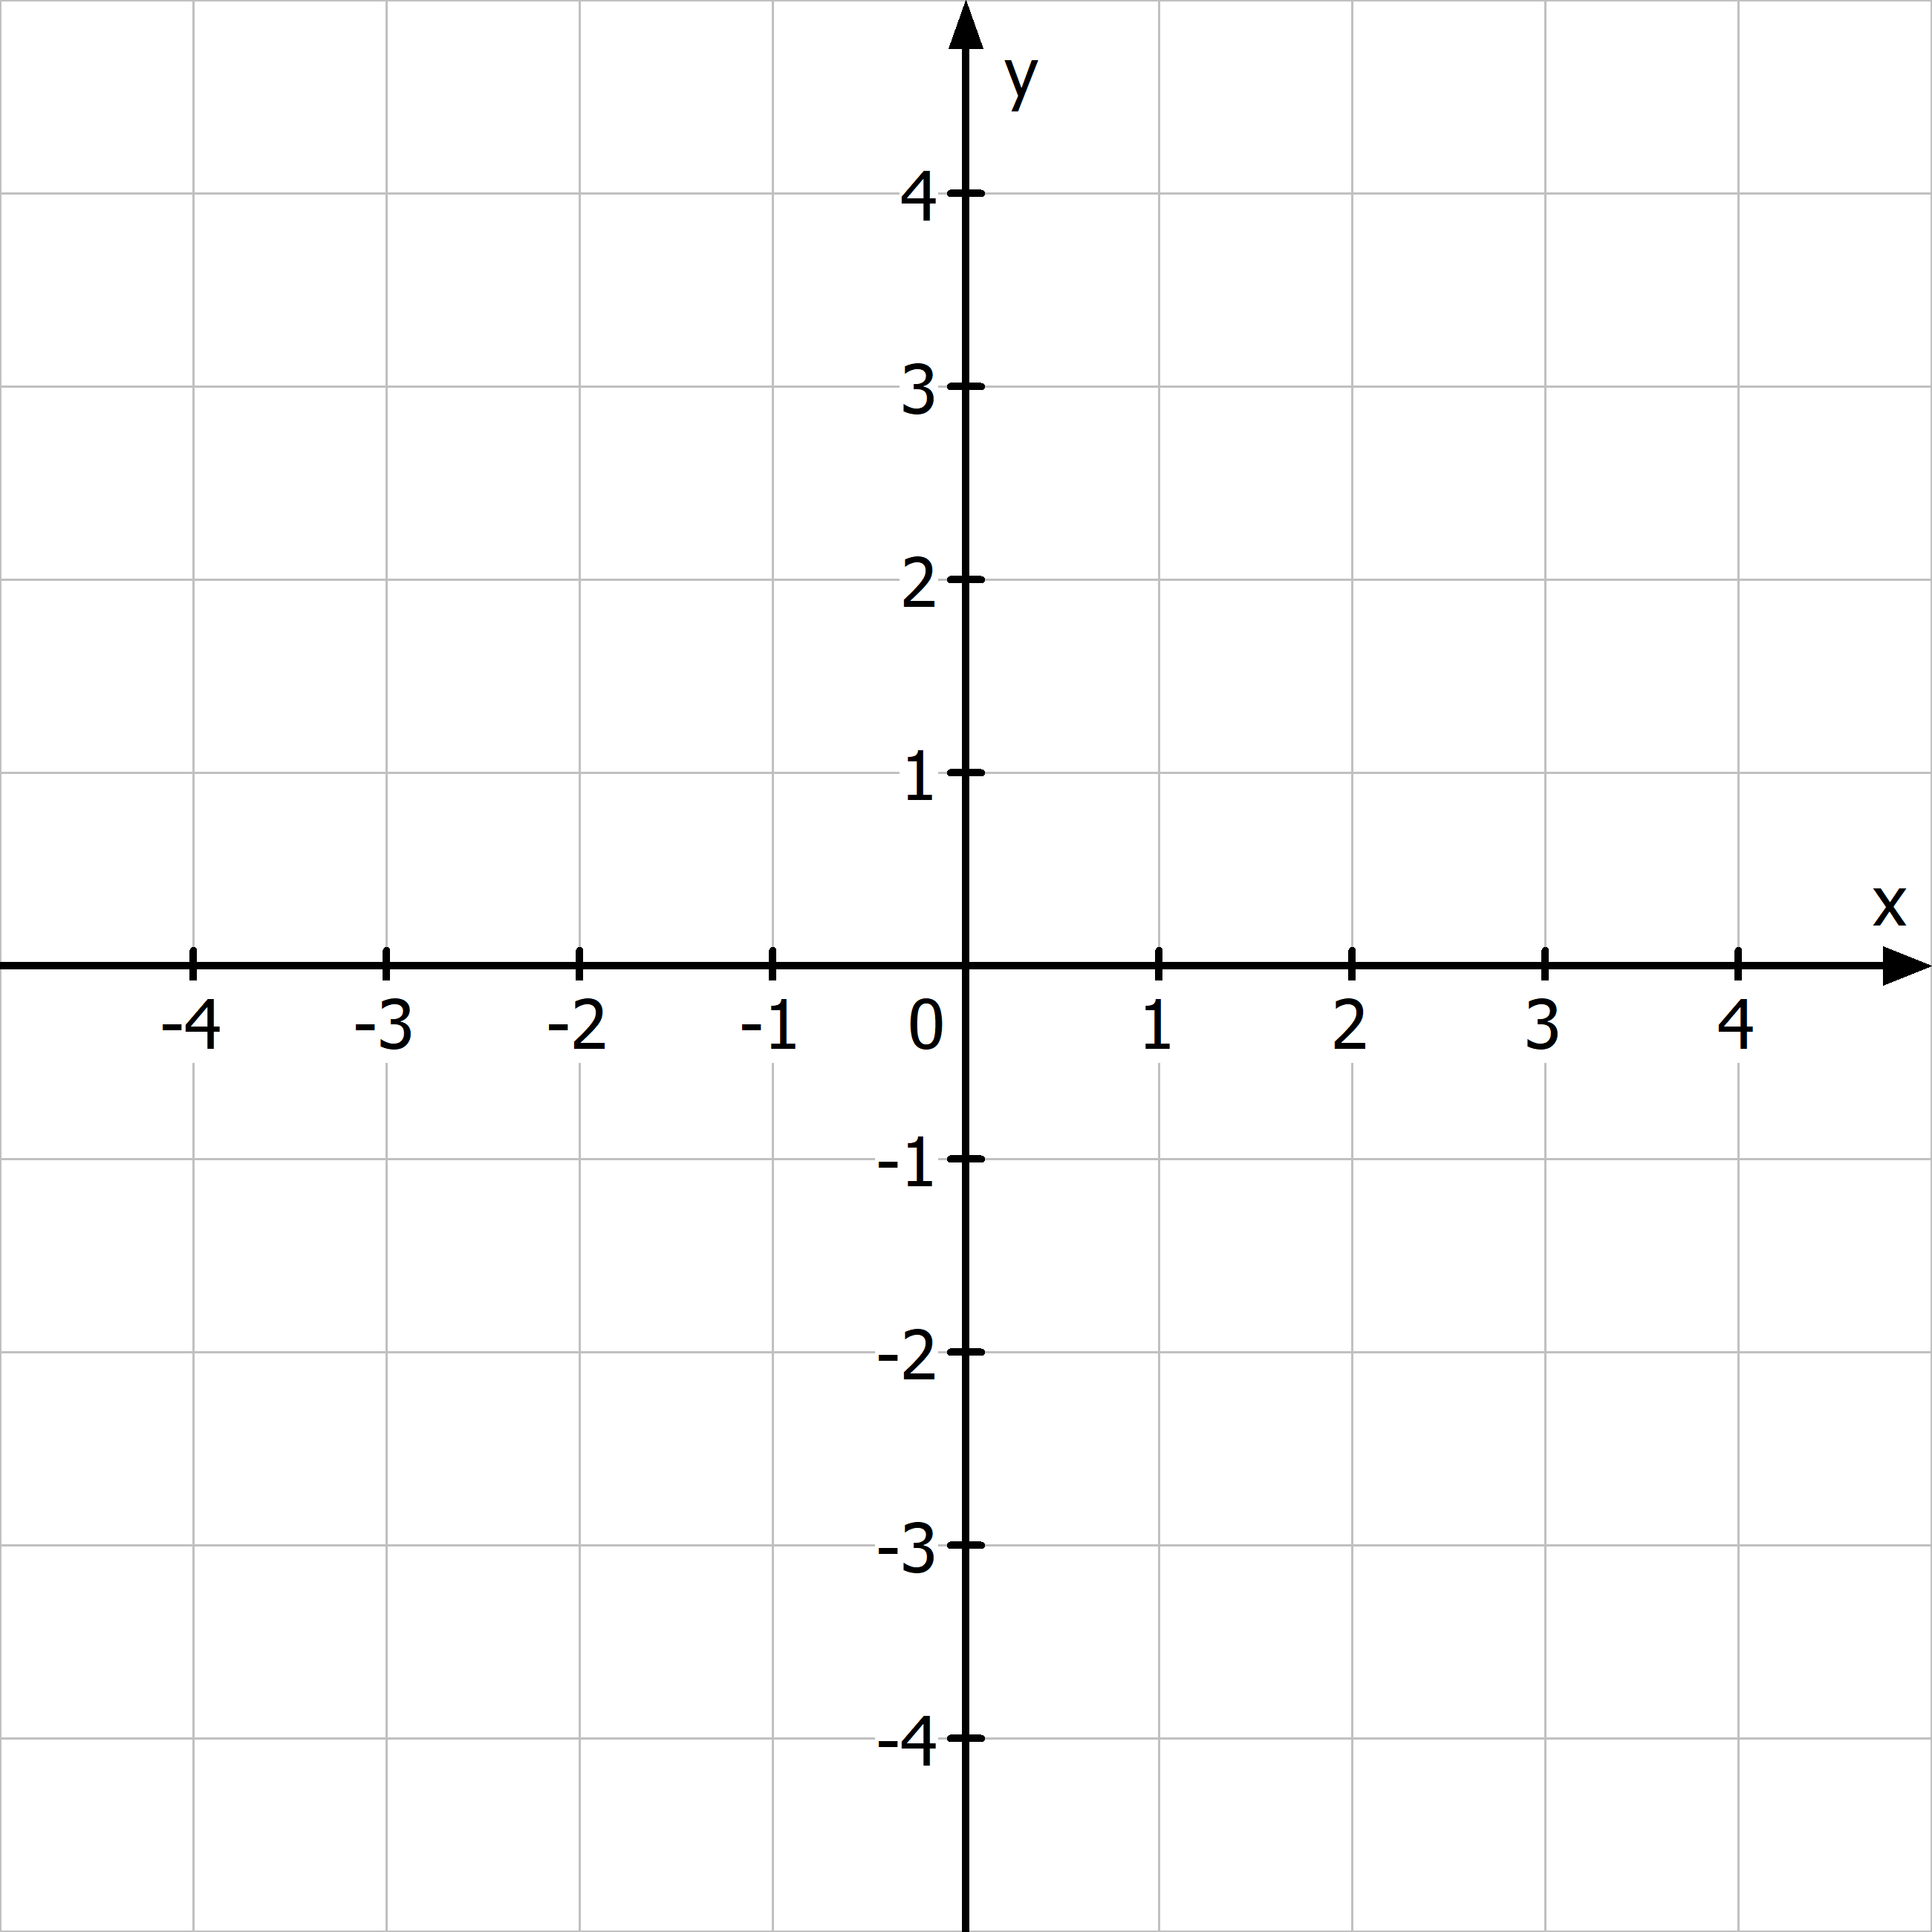
\includegraphics[width=\linewidth]{\linFkt/pics/lage_empty.png}}}

		\(f_1(x)=\tfrac{1}{2}x-2\qquad g_1(x)=0,5x+1\)
	\end{minipage}}%
	\adjustbox{valign=t, padding=2ex 0ex 0ex 0ex}{\begin{minipage}{0.5\linewidth-2ex}\centering
		\begin{tcolorbox}[width=\linewidth, height=1.2cm, valign=center]\centering
			\textcolor{loestc}{\(m_f=m_g\)}
		\end{tcolorbox}
		\raggedright
		\textcolor{loes}{Die beiden Geraden haben die gleiche Steigung. Solche Paare von Geraden nennt man parallele Geraden. Sie haben keinen Schnittpunkt, d.h. die Gleichung \(f(x)=g(x)\) hat keine Lösungen. Paralle Geraden, die auch den gleichen y-Achsenabschnitt haben, nennt man identische Geraden. In diesem Fall ist jedes \(x\) eine Lösung der Gleichung \(f(x)=g(x)\)}.
	\end{minipage}}%
\end{minipage}

\bigskip

\begin{minipage}{\textwidth}
	\adjustbox{valign=t, padding=0ex 0ex 2ex 0ex}{\begin{minipage}{0.5\linewidth-2ex}
		\centering{\Large\textcolor{loes}{Senkrechte Geraden}}
	\end{minipage}}%
	\adjustbox{valign=t, padding=2ex 0ex 0ex 0ex}{\begin{minipage}{0.5\linewidth-2ex}
		\centering{\Large\textcolor{loes}{keine besondere Lage}}
	\end{minipage}}%
\end{minipage}%

\begin{minipage}{\textwidth}
	\adjustbox{valign=t, padding=0ex 0ex 2ex 0ex}{\begin{minipage}{0.5\linewidth-2ex}
			\centering{\iftoggle{ausfuellen}{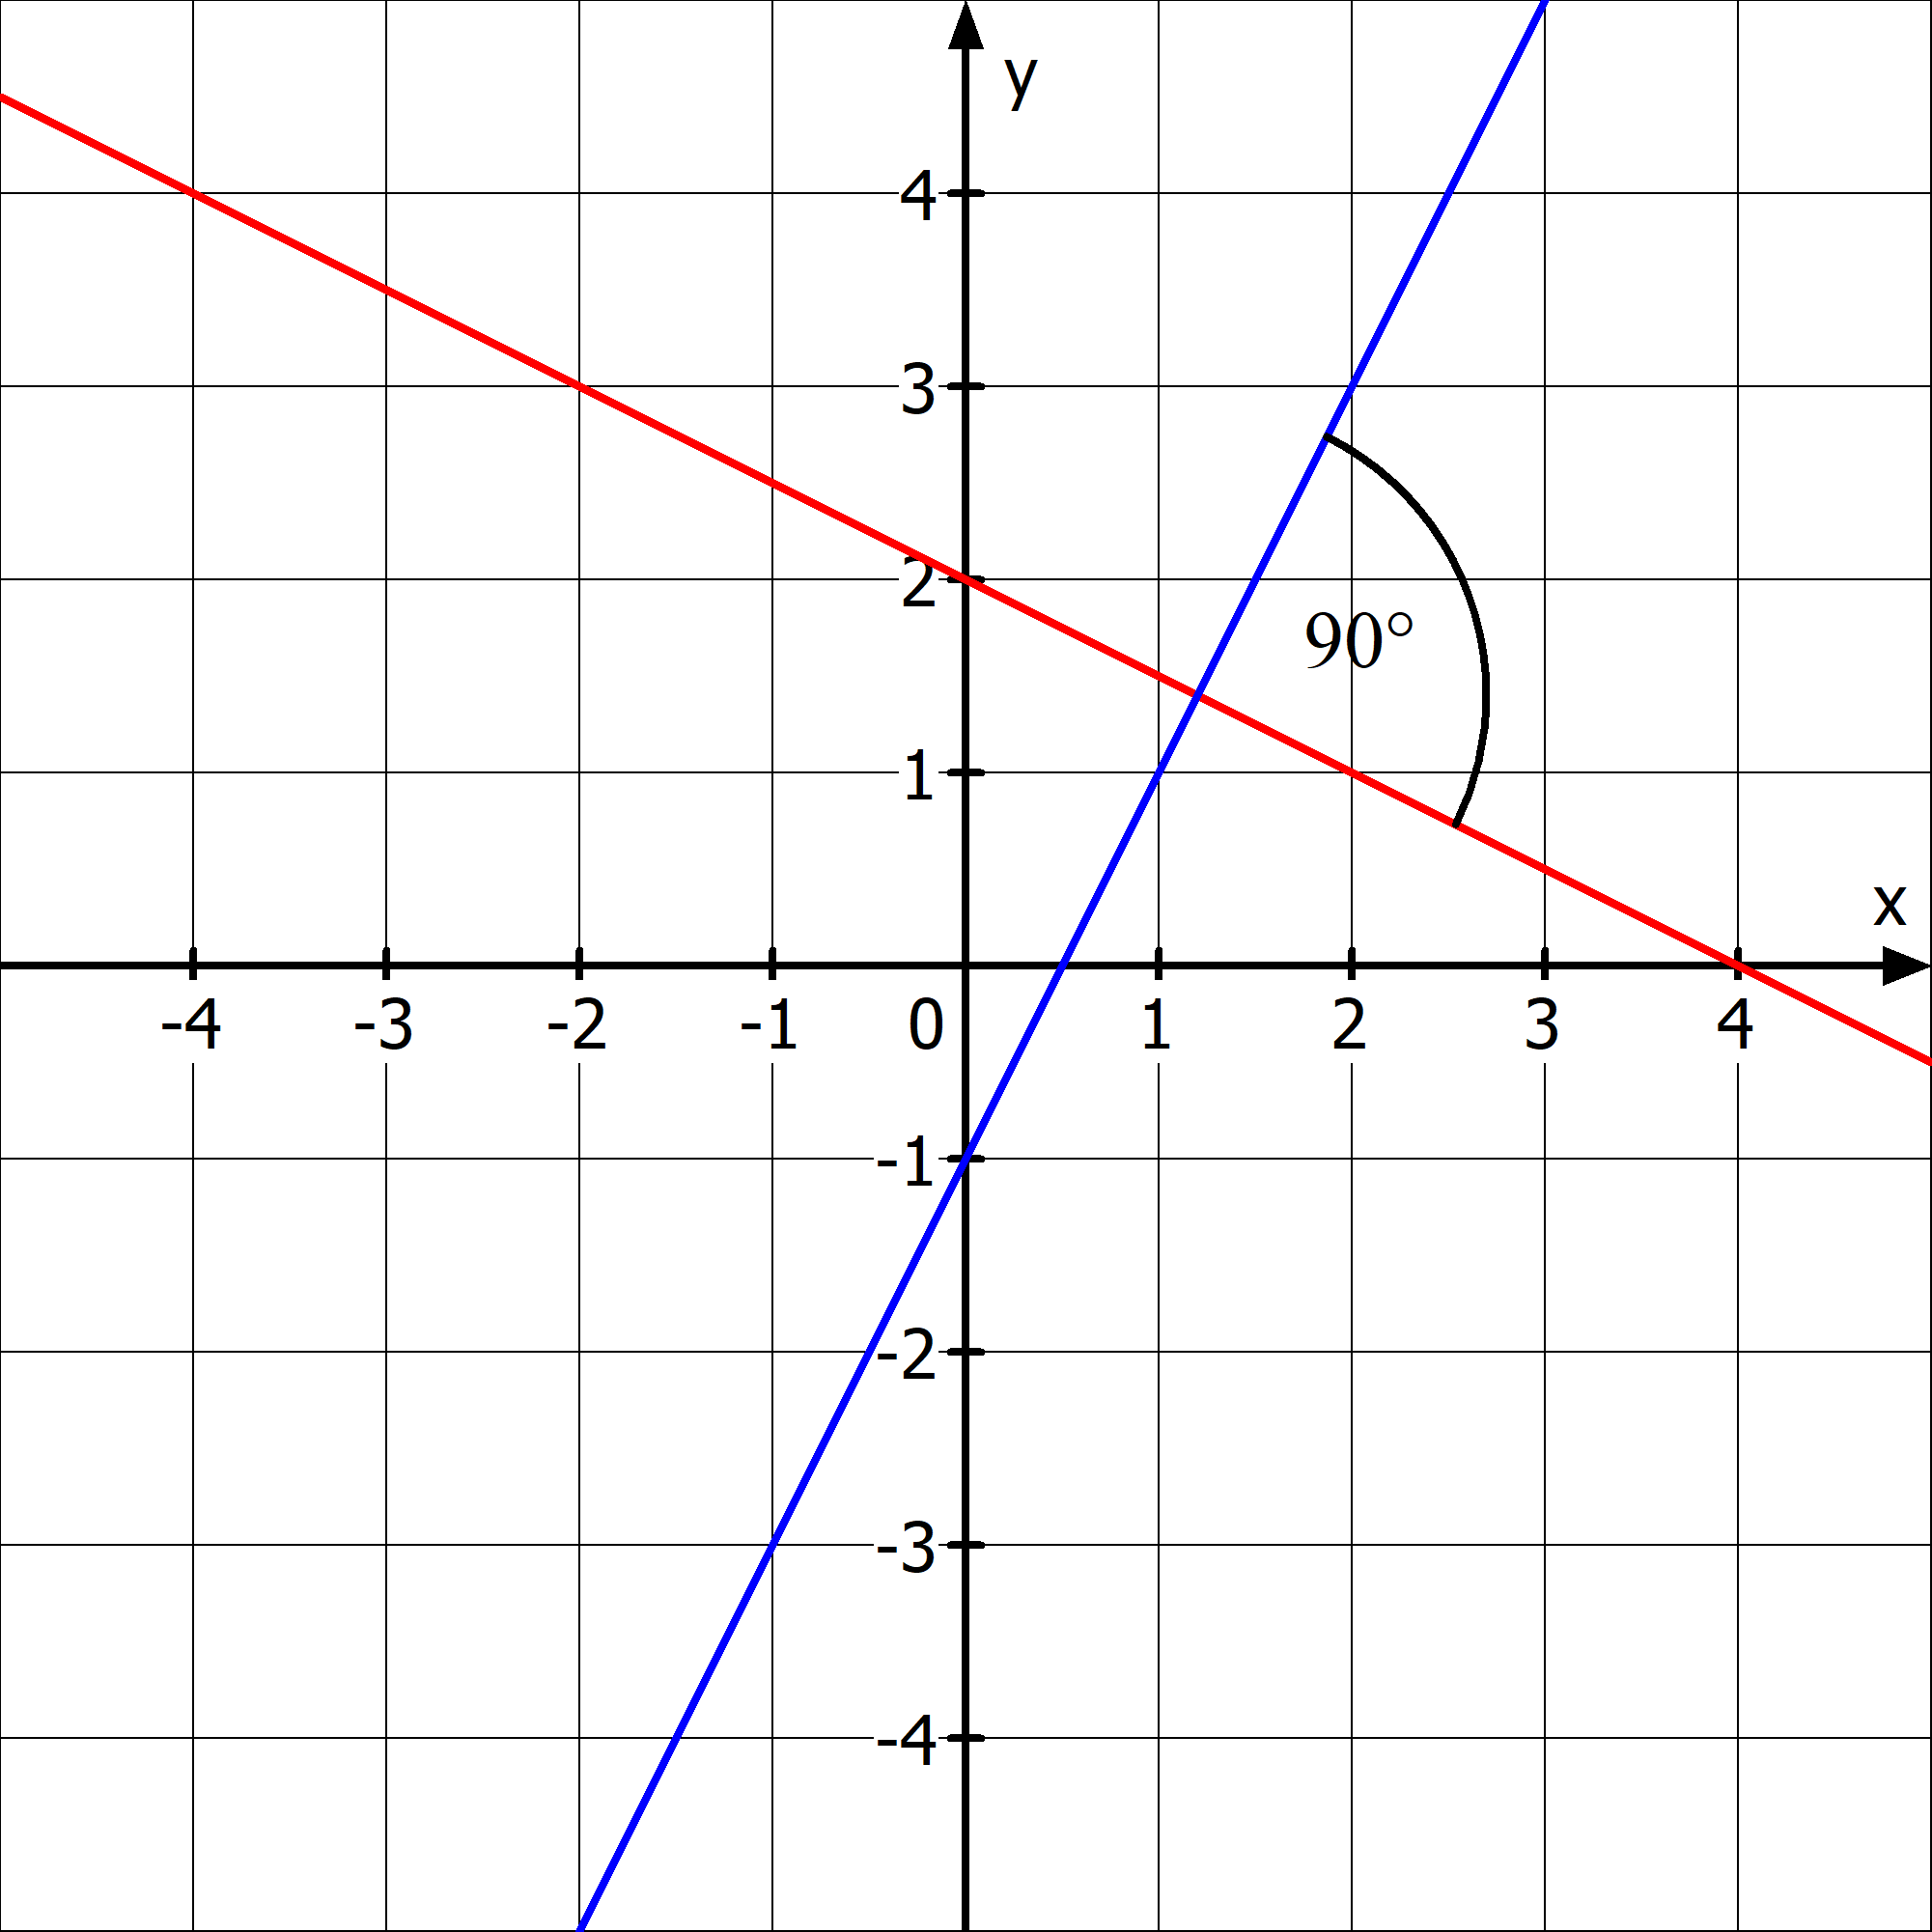
\includegraphics[width=\linewidth]{\linFkt/pics/lage2.png}}{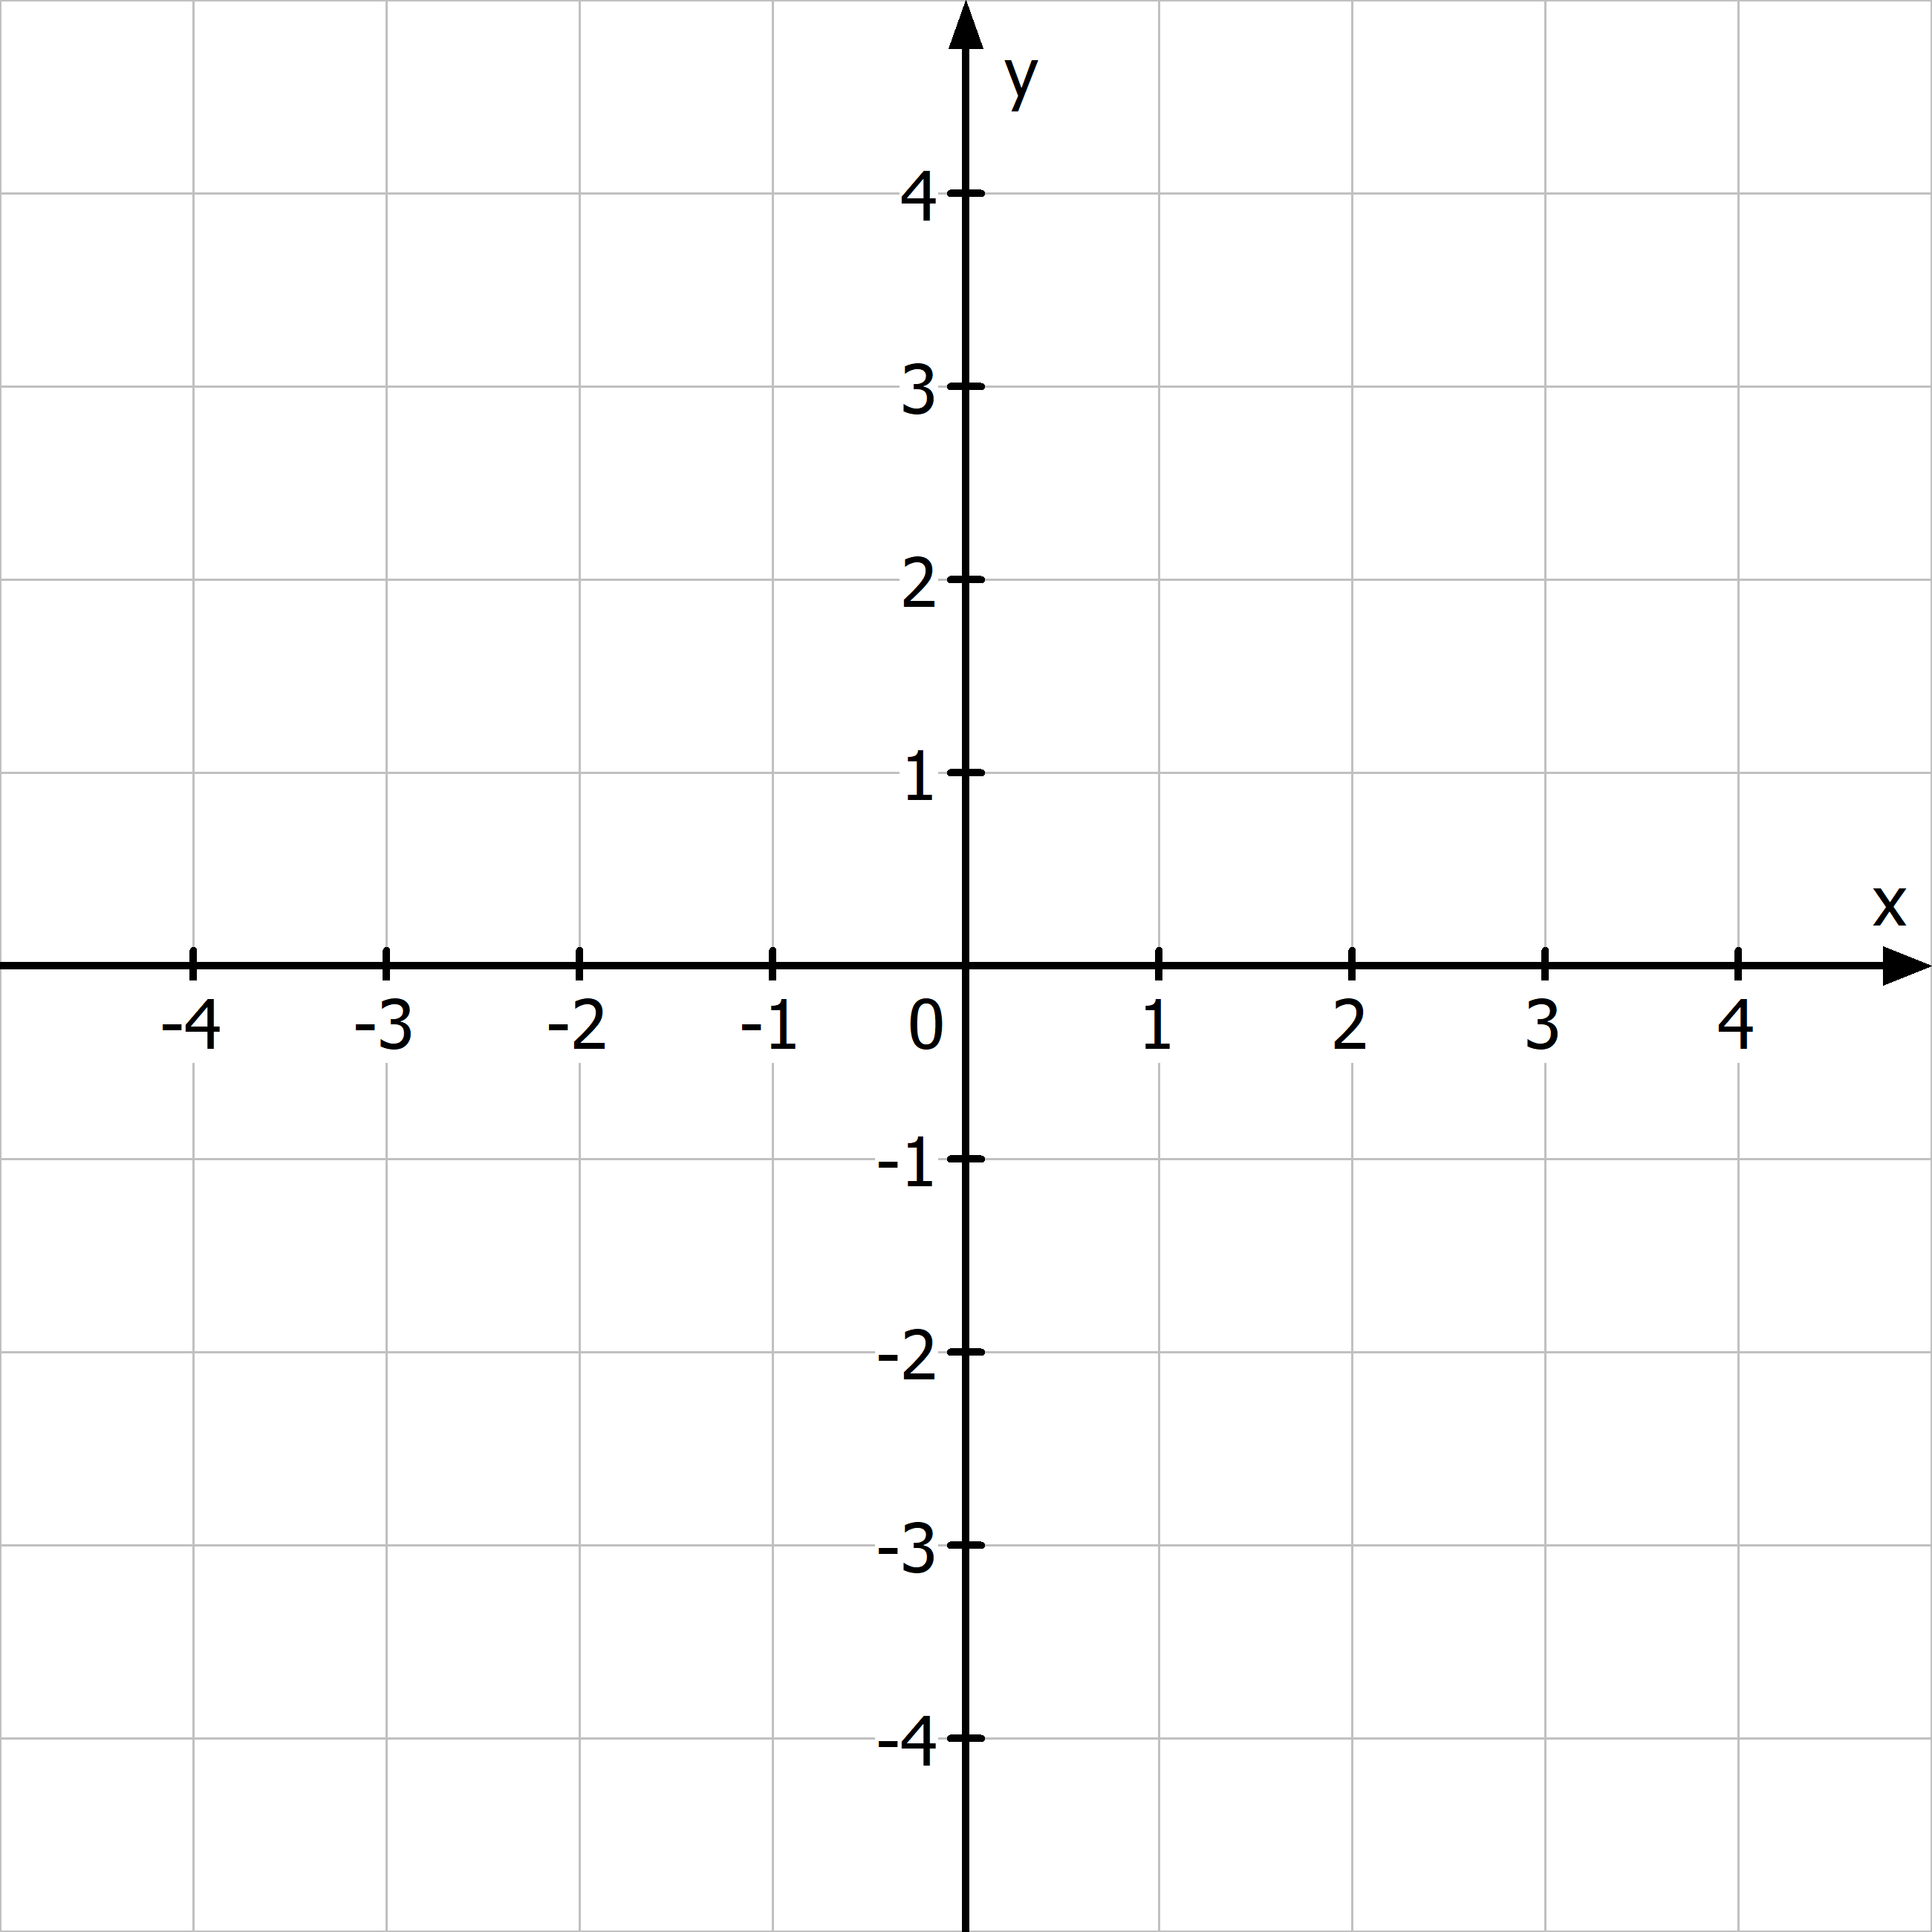
\includegraphics[width=\linewidth]{\linFkt/pics/lage_empty.png}}}
	\end{minipage}}%
	\adjustbox{valign=t, padding=2ex 0ex 0ex 0ex}{\begin{minipage}{0.5\linewidth-2ex}
			\centering{\iftoggle{ausfuellen}{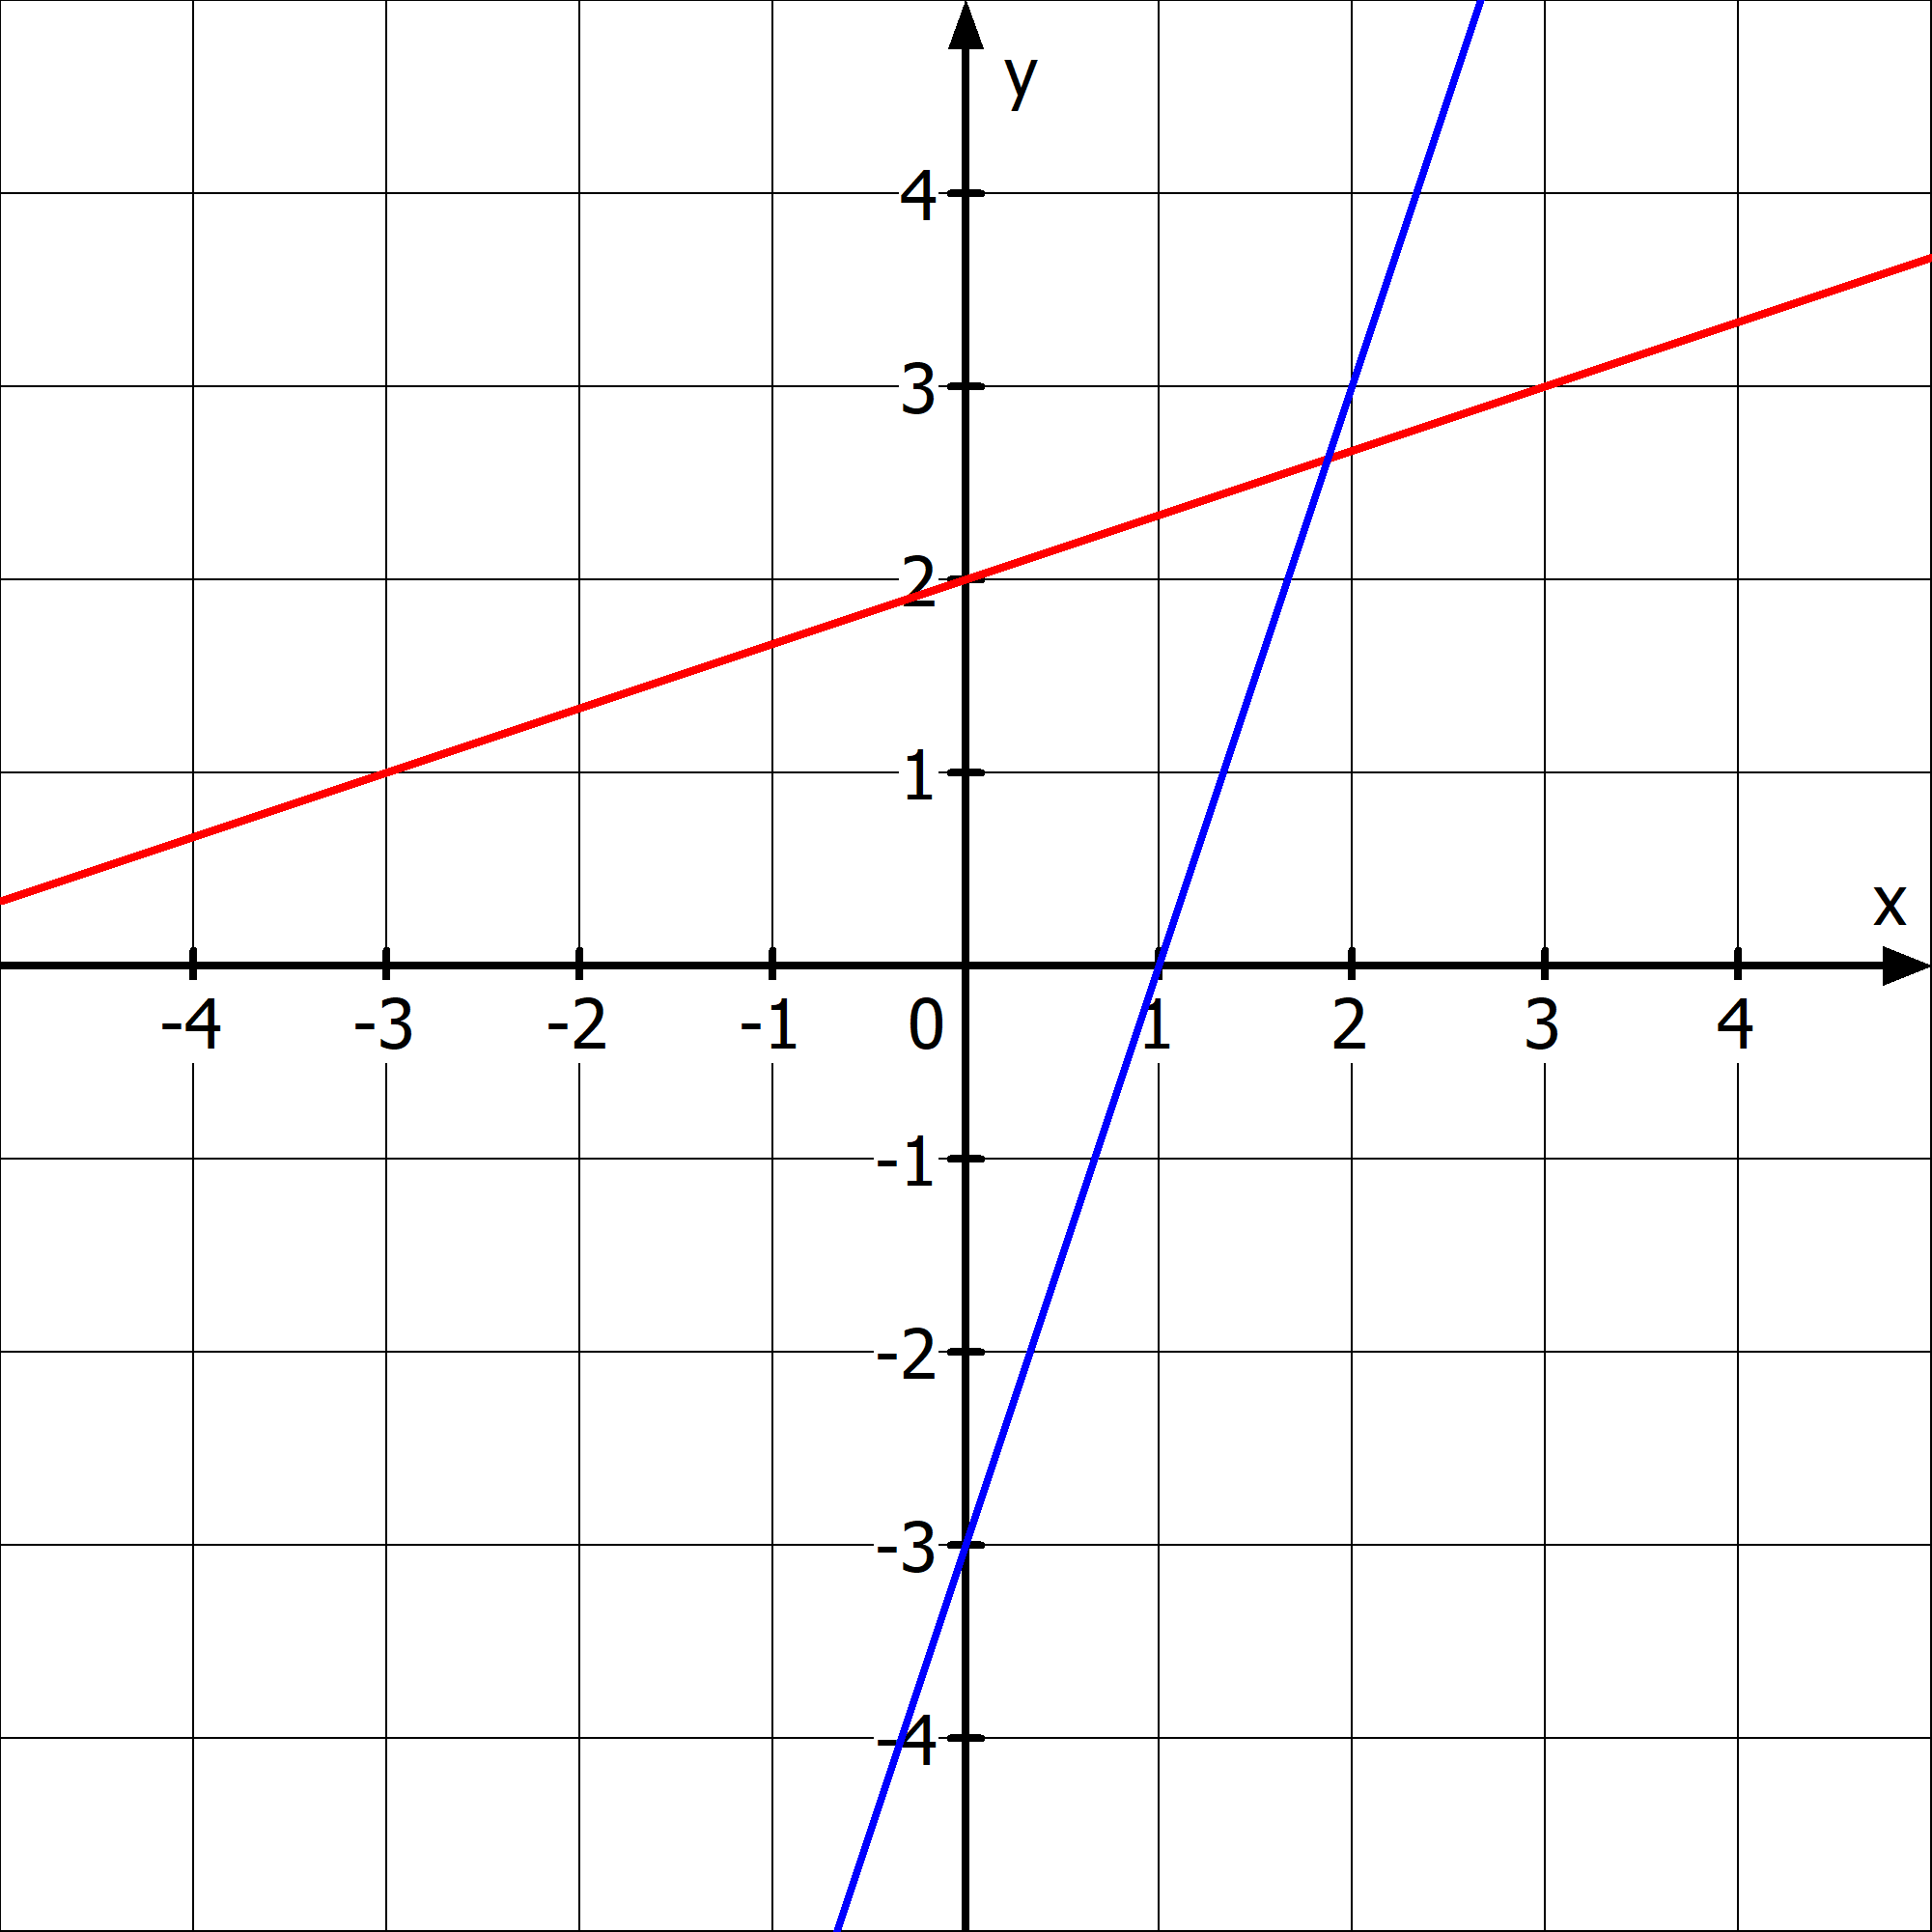
\includegraphics[width=\linewidth]{\linFkt/pics/lage3.png}}{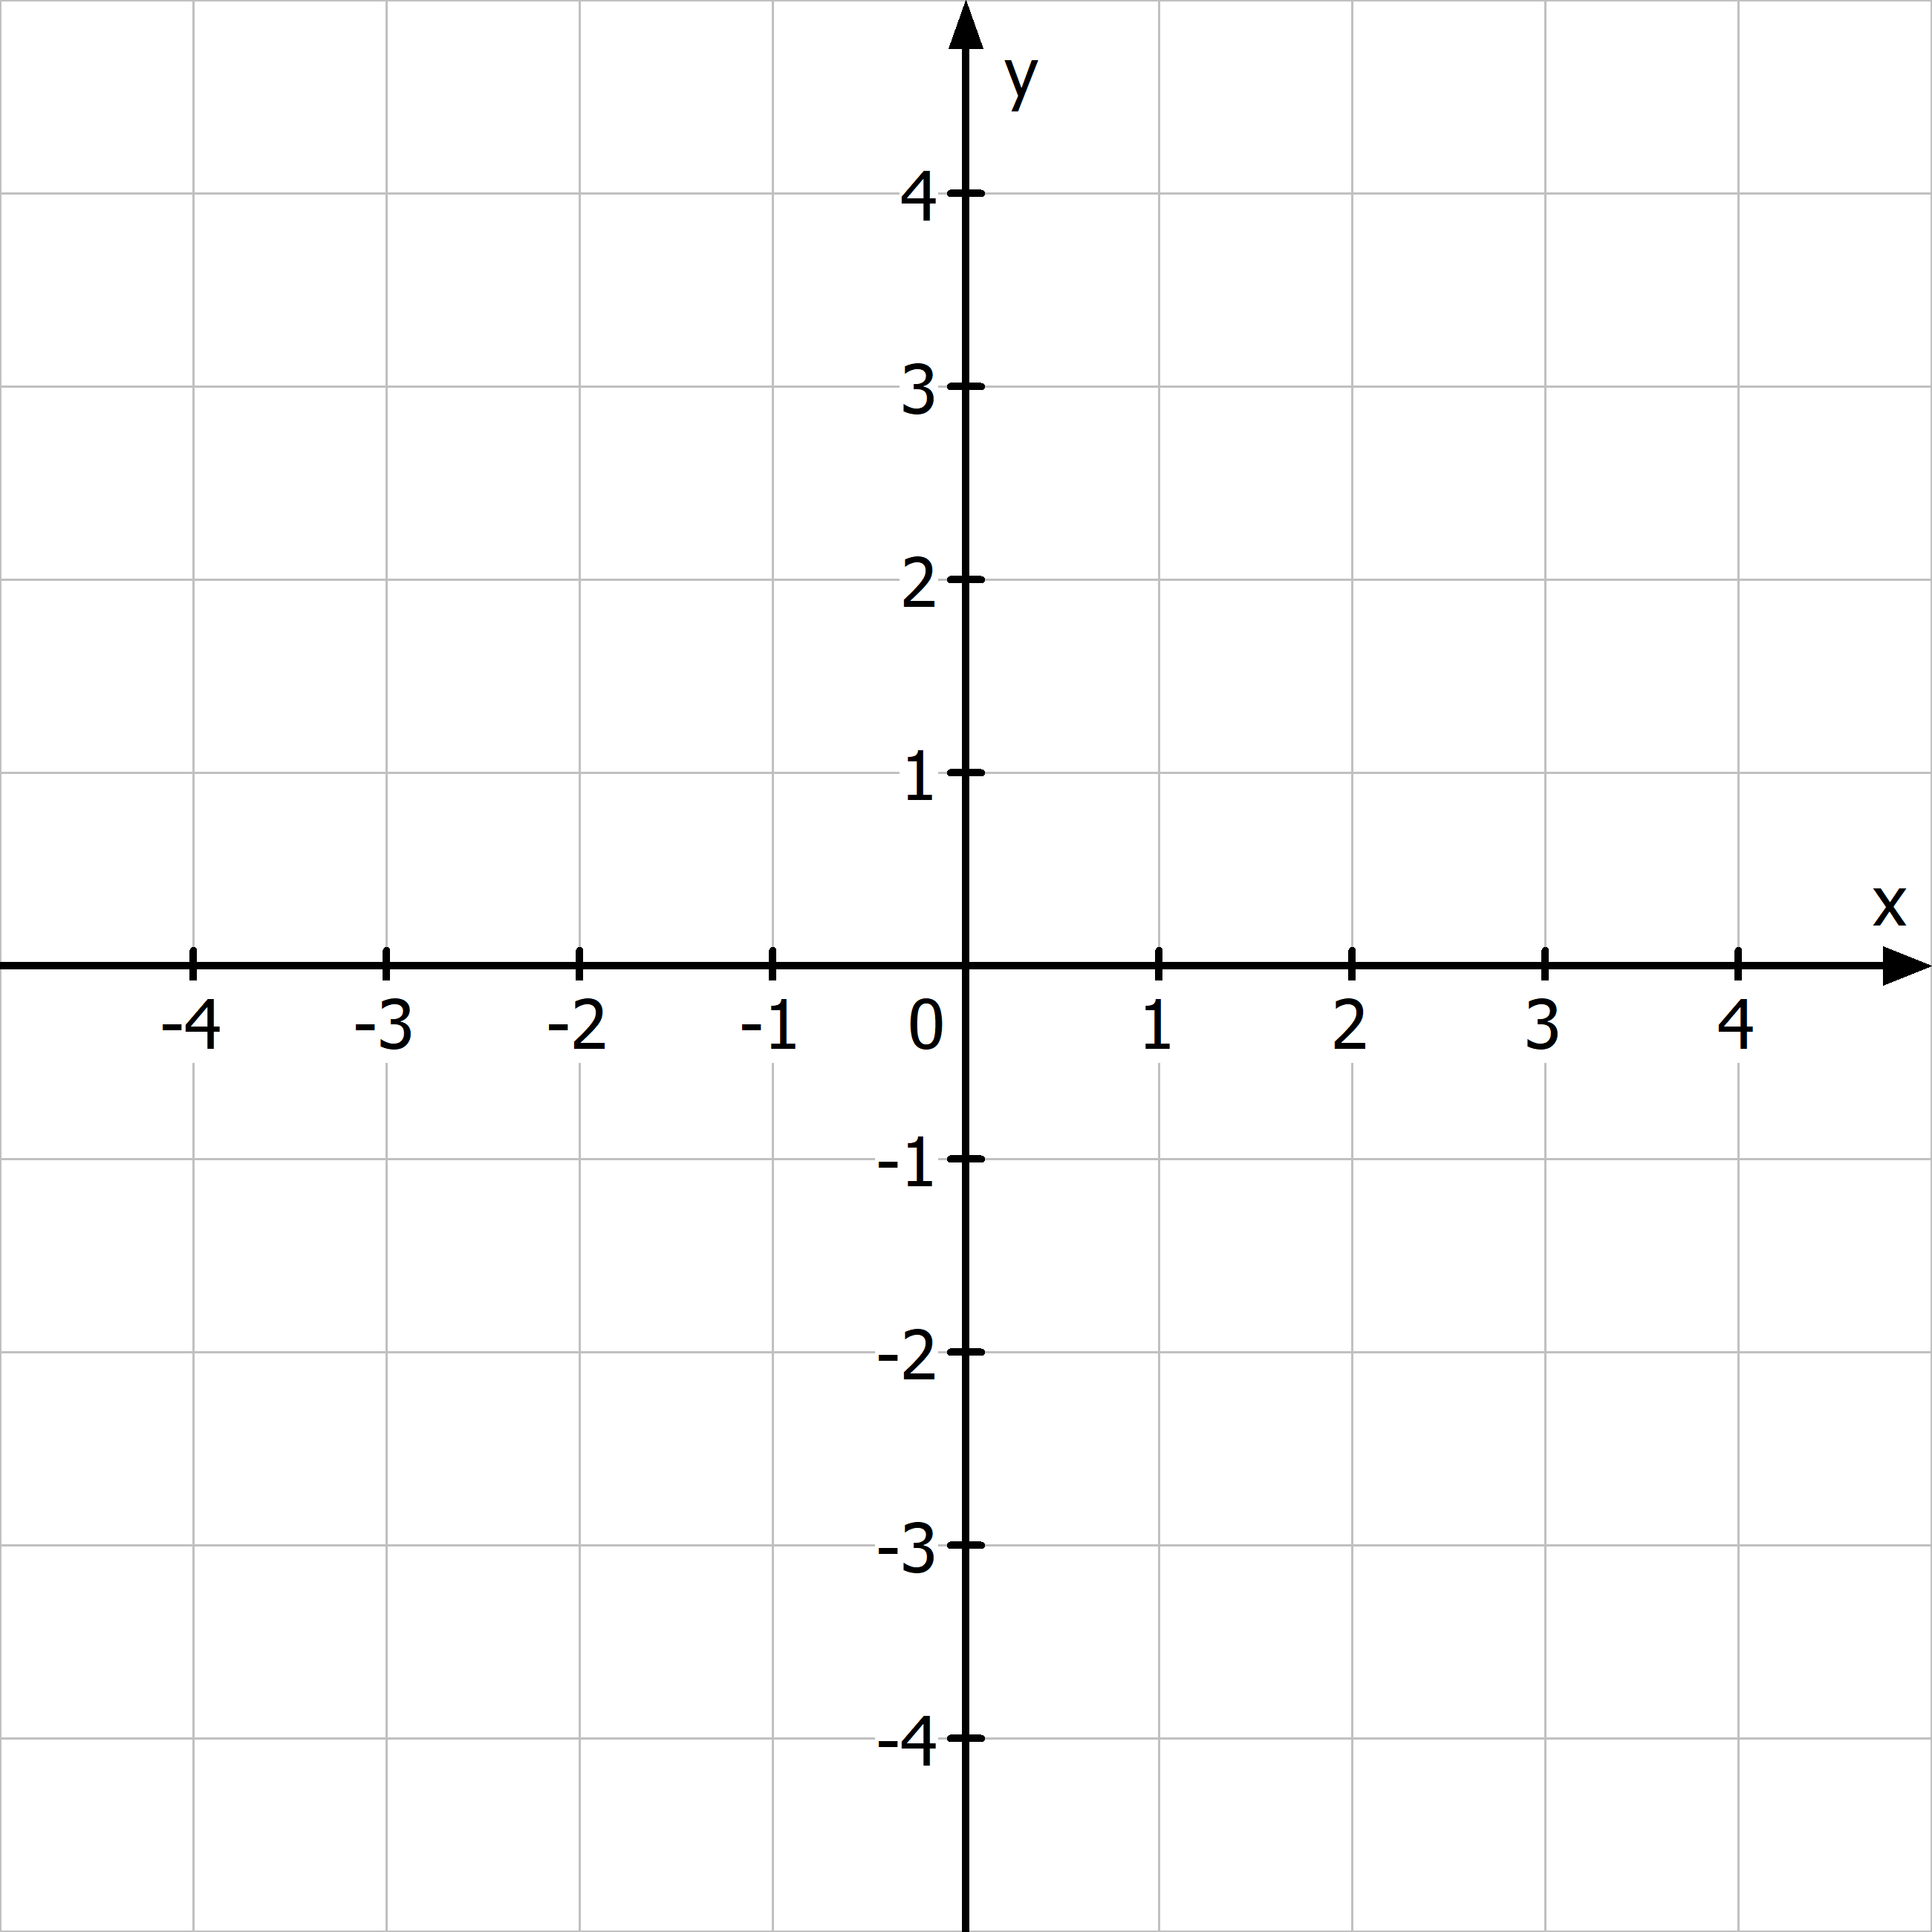
\includegraphics[width=\linewidth]{\linFkt/pics/lage_empty.png}}}
	\end{minipage}}%
\end{minipage}%

\bigskip

\begin{minipage}{\textwidth}
	\adjustbox{valign=t, padding=0ex 0ex 2ex 0ex}{\begin{minipage}{0.5\linewidth-2ex}
			\centering\(f_2(x)=-\tfrac{1}{2}x+2\qquad g_2(x)=2x-1\)
	\end{minipage}}%
	\adjustbox{valign=t, padding=2ex 0ex 0ex 0ex}{\begin{minipage}{0.5\linewidth-2ex}
			\centering\(f_3(x)=\tfrac{1}{3}x+2\qquad g_3(x)=3x-3\)
	\end{minipage}}%
\end{minipage}%

\bigskip

\begin{minipage}{\textwidth}
	\adjustbox{valign=t, padding=0ex 0ex 2ex 0ex}{\begin{minipage}{0.5\linewidth-2ex}\centering
			\begin{tcolorbox}[width=\linewidth, height=1.2cm, valign=center]\centering
				\textcolor{loestc}{\(m_f\cdot m_g=-1\)}
			\end{tcolorbox}
	\end{minipage}}%
	\adjustbox{valign=t, padding=2ex 0ex 0ex 0ex}{\begin{minipage}{0.5\linewidth-2ex}\centering
			\begin{tcolorbox}[width=\linewidth, height=1.2cm, valign=center]\centering
				\textcolor{loestc}{\(m_f\neq m_g\textbf{ und }m_f\cdot m_g\neq-1\)}
			\end{tcolorbox}
	\end{minipage}}%
\end{minipage}%

\bigskip

\begin{minipage}{\textwidth}
	\adjustbox{valign=t, padding=0ex 0ex 2ex 0ex}{\begin{minipage}{0.5\linewidth-2ex}
			\raggedright
			\textcolor{loes}{Die beiden Geraden schneiden sich in einem rechten Winkel. Solche Paare von Geraden stehen orthogonal bzw. normal zueinander.}
	\end{minipage}}%
	\adjustbox{valign=t, padding=2ex 0ex 0ex 0ex}{\begin{minipage}{0.5\linewidth-2ex}
			\raggedright
			\textcolor{loes}{Die beiden Geraden sind weder parallel noch orthogonal, d.h. sie haben keine besondere Lage zueinander.}
	\end{minipage}}%
\end{minipage}%